\chapter{Introducción}

La democratización de Internet ha hecho que hoy día, al igual que en otras materias, sea impensable concebir la enseñanza sin hacer uso de Internet, tanto para la búsqueda de información como para la comunicación profesor-alumno y es posible que en el futuro la totalidad de la enseñanza se imparta a través de la red.

\bigskip
Aunque a efectos legales la labor de un profesor tenga un horario establecido (posiblemente de 8.00 a 15.00 horas), uno no deja de ser profesor, de hecho la mayoría de los profesores ejercen la profesión 24 horas al día, 7 días a la semana durante los 365 días del año. Dicha dedicación, que es en gran medida vocacional nos puede llegar a consumir gran parte de nuestro tiempo y por eso tenemos que apoyarnos en metodologías que nos permitan optimizar nuestro tiempo a la vez que permitan transmitir conocimientos de una forma exponencial. Imaginemos que podamos enseñar programación a 500 alumnos a la vez con la misma calidad que la que podemos dar en una tutoría personalizada ¿no sería fantástico?. Puede sonar utópico e irrealizable pero como dice Richard Branson: ``If your dreams don’t scare you, they are too small''. Con las herramientas adecuadas, haciendo uso de la automatización podemos adaptar la metodología ``Exponential Organizations'' (\cite{ismail_exponential_2014}) al mundo de la enseñanza. De hecho conceptos como el ``ExO Sprint'' de 10 semanas (\cite{ismail_exponential_2018}) se puede usar para optimizar nuestra forma de impartir clase.

\bigskip
Durante mis años de estudiante conocí a profesores que se limitaban a repetir año tras año la misma teoría, con unos ejercicios copiados de algún sitio de Internet sin tan siquiera plantearse que sus futuros alumnos también tendrían acceso a Internet y sabrían buscar la fuente original de dichos ejercicios, pero a su vez también tuve profesores que coqueteaban con todo tipo de nuevas tecnologías para mejorar su labor docente, y sirviendo dicho coqueteo para mantenerse actualizados en cuanto a las nuevas tecnologías que han ido apareciendo. Estos últimos han sido los que me han motivado tanto a llegar a ser profesor como a intentar mejorar dentro de mis posibilidades las metodologías de enseñanza de la programación.


\section{Motivación}

Como ya he comentado en ocasiones anteriores (\cite{ernesto_prado_2016}) mi primer contacto con la informática fue a finales de los ochenta. Un buen día mi padre apareció en casa con una caja que contenía un rudimentario teclado negro con un arco-iris serigrafiado. Ese mismo teclado tenía una ranura para introducir cintas de casete como las que servían para escuchar música y tras esperar lo que ahora nos parecería una eternidad podíamos empezar a aporrear el teclado para llevar a Phantomas (figura \ref{fig:phantomas}) de pantalla en pantalla mientras íbamos esquivando enemigos y activando las palancas que abrirían la caja fuerte de la mansión que íbamos a robar.


\begin{figure}[h!]
\centering
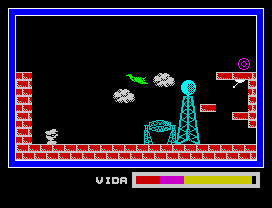
\includegraphics{../images/phantomas-sp1}
\caption{Phantomas (© 1986 Dinamic)}
\label{fig:phantomas}
\end{figure}

\bigskip
Todavía faltaba mucho tiempo para que aprendiera lo que era una interfaz (aún no había aprendido apenas a leer) pero ya sabía interpretar algunas letras, curiosamente las que tenían pintadas las teclas OPQA\footnote{En los primeros ordenadores de la década de los 80 OPQA era la combinación de teclas que usaban la mayoría de los juegos siendo OP las teclas para moverse de izquierda a derecha y QA para hacerlo de arriba a abajo.}.

\bigskip
Según fui creciendo aprendí a leer y escribir y también a diferenciar entre texto y código, para mí el código eran un serie de letras que aparecían impresas en las últimas páginas de las revistas que compraba mi hermano. Esos códigos se llamaban POKES\footnote{Instrucción en lenguaje BASIC para guardar un valor en una dirección de memoria.}, y cuando los introducías en un juego conseguías cosas como vidas infinitas, la habilidad de atravesar paredes o la capacidad de ser invisible a los enemigos.

\bigskip
Algunos años mas tarde aparecieron las consolas de videojuegos en las que metías un cartucho e instantáneamente estabas jugando a juegos increíbles con una paleta de colores que raro era que no provocara ataques epilépticos. Mientras mis amigos solo tenían que introducir el cartucho y empezar a jugar yo tenía que esperar 5 interminables minutos mientras escuchaba sonidos estridentes y cruzar los dedos por que no apareciera el fastidioso TAPE ERROR que se podía intentar solucionar girando un tornillo llamado ``azimut'' con un destornillador de estrella.

\bigskip
Y de esta manera, sin siquiera saberlo, tuve mis primeros contactos con el auto-aprendizaje, yo girando un tornillo sin saber a ciencia cierta el por qué y cuando el mayor problema que tenían mis amigos era que a veces tenían que dar un soplido fuerte al cartucho.

\bigskip
Pasaron los años, los sistemas se fueron haciendo mas complejos y me di cuenta de que cuantas más opciones tenían los dispositivos, más perezosos se volvían los usuarios. Mi vecino sin ir más lejos, por no aprender a ajustar su televisor tenía ``La 2'' en el canal 3 ¿era yo el único que encontraba eso chirriante? Quizá no, pero como he ido descubriendo hay diferentes tipos de personas, están los que pueden pasar meses alumbrando el pasillo con el teléfono móvil y los que crean un tutorial en YouTube para enseñar a cambiar una bombilla.

\bigskip
Y ese es el deber que tenemos como futuros profesores, ser capaces de transmitir ese conocimiento e intentar que nuestros alumnos no pasen meses a oscuras, que aprendan a silenciar el volumen del altavoz del módem y en el mejor de los casos que sepamos despertar en ellos la curiosidad para que sean ellos mismos los que auto-aprendan y descubran todas esas cosas futuras que aun siendo profesores tenemos por aprender.

\section{Definición del problema}

Este proyecto intentará abordar los siguientes objetivos:

\begin{itemize}
  \item Reducir la tediosa tarea de la corrección de ejercicios.
  \item Motivar la enseñanza y aprendizaje de la programación a través de ejemplos.
  \item Ver las ventajas de usar sistemas de control de versiones.
  \item Enseñar a nuestros alumnos como utilizar un sistema de control de versiones de forma correcta.
  \item Mostrar nuevas prácticas de programación como puede ser la integración continua.
\end{itemize}

\section{Estructura del proyecto}


\bigskip
Antes de pasar a detalles más técnicos, me gustaría detallar el contenido de este proyecto:

\begin{itemize}
  \item En el \textit{capítulo 1} (\textbf{Introducción}) se encuentra una una breve introducción a nuestra idea así como las motivaciones que nos han llevado a realizarla.
  \item El \textit{capítulo 2} (\textbf{Objetivos}) detalla de forma algo más concreta los objetivos determinados que se quieren cumplir con este proyecto.
  \item En el \textit{capítulo 3} (\textbf{Antecedentes}) se analiza el estado de arte actual, así como algunas de las tecnologías y paradigmas que utilizaremos en nuestro proyecto.
  \item En el \textit{capítulo 4} (\textbf{Propuesta pedagógica}) se analizan los detalles pedagógicos del proyecto.
  \item En el \textit{capítulo 5} (\textbf{Propuesta metodológica}) se planifica cómo se van a realizar de forma técnica los contenidos del proyecto.
  \item En el \textit{capítulo 6} (\textbf{Conclusiones}) se pueden encontrar las conclusiones finales así como las recomendaciones para futuros trabajos.

\end{itemize}


\bigskip
Para finalizar se incluye un anexo con el código fuente desarrollado y liberado bajo la licencia libre \cite{gplv3}. Dicho código fuente se puede encontrar en la url \url{https://github.com/erseco/ugr_tfm_maes_sample_exercises/}.


% %
% % Ejemplos de codigo LaTeX para uso futuro
% %

% \begin{figure}[h!]
% \centering
% 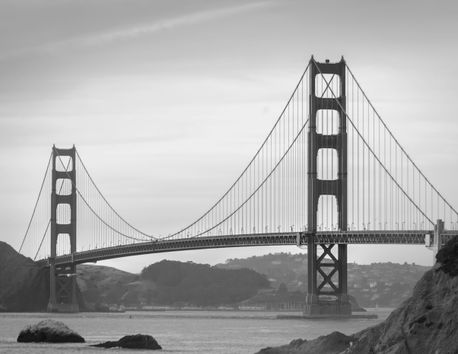
\includegraphics{../screenshots/sample1}
% \caption{Sample Image 1}
% \label{fig:sample1}
% \end{figure}

% Esto es un texto con una nota\footnote{Ejemplo de nota al pie} al pie.

% Y esto es una ``Frase de alguien''\cite{stevekrug}.

% \begin{itemize}
%   \item \textbf{1.} Texto de ejemplo
%   \item \textbf{2.} Texto de ejemplo
%   \item \textbf{3.} Texto de ejemplo
%   \item \textbf{4.} Texto de ejemplo

% \end{itemize}

% \begin{enumerate}
% 	\item Ejemplo 1.
% 	\item Ejemplo 2.
% \end{enumerate}

% \begin{lstlisting}[language=html]
% <!DOCTYPE html>
% <html lang="es-ES">
%   <head>
%     <meta charset="utf-8">
%     <title>Ejemplo de 2 párrafos</title>
%   </head>
%   <body>
%     <p>Esto es un párrafo.</p>
%     <p>Esto es otro párrafo.</p>
%   </body>
% </html>
% \end{lstlisting}

% Puedes verlo en \cite{Patricio2011}. Te recomiendo leer \cite{Patricio2011, Zacarias2009, Alfonso2010b, Alfonso2010a}.
